% !TEX root = main.tex

\section{Entwurf}
%Hier sollten noch Abbildungen und/oder Schemen hinzugefügt werden --> Klassendiagramm??? Wäre wahrscheinlich falsch, weil C
\subsection{Variantenaufbau}
Um die verschiedenen Implementierungen möglichst unabhängig voneinander zu testen, haben wir uns dazu entschieden drei separate Programme zu entwickeln. Die sequentielle Variante unterscheidet sich dabei nur gering von der OpenMP-Variante. Die OpenMPI hat jedoch deutliche Unterschiede. Letzteres benötigt zudem einen speziellen Compiler und einen spezielles Programm zum Ausführen. Dies war auch ein Grund für die strikte Trennung der Varianten.\\
Da die verwendeten Frameworks pimär in der Programmiersprache C vorliegen und diese teilweise auch so in der Vorlesung vorgestellt wurden, haben wir uns auch für diese Sprache entschieden.

\subsection{Programmaufbau}
C ist eine prozedurale Programmiersprache, d.h. es gibt keine Klassen. Wir haben jedoch unsere Klassenstruktur in Anlehnung an diese entworfen. Dabei unterteilen wir jedes Programm in drei Teile, welche aus jeweils zwei Dateien bestehen (C-Datei und Header-Datei): wave, config und core.

\subsubsection{wave.c / wave.h}
Hier findet die Programminitialisierung und hier sind auch alle Methoden und Variablen, die für die grafische Benutzeroberfläche (GUI) verwendet werden, angesiedelt. Für die GUI haben wir uns für das GTK-Framework entschieden. Die einzige Vorgabe die wir uns hier zunächst gemacht haben, ist dass die GUI möglichst wie die Vorgabe aus der Aufgabenstellung aussehen soll. Da es in dieser Arbeit um die Parallelisierung gehen soll, werden wir nicht auf Details eingehen.\\
Die anderen Programmteile werden von hier aus aufgerufen, d.h. der gesamte Programmfluss findet im Prinzip hier statt bzw. wird von hier gesteuert.

\subsubsection{core.c / core.h}
Hier findet die Logik des Programms statt. Hier liegen drei Arrays die den Verlauf der Welle darstellen. Dabei stellt eins die Vergangenheit, eins die Gegenwart und eins die Zukunft dar. Die Arrays der Vergangenheit und der Gegenwart werden initial mit einer Sinuskurve beschrieben. Wobei eine der Sinuskurven eine Verschiebung aufweisen kann, sodass eine Dynamik in der Animation entsteht.\\
Die Werte der Zukunft werden dann immer mithilfe der in Abschnitt \ref{sec:wave_equation} vorgestellten Gleichung und den Werten der Gegenwart und der Vergangenheit berechnet. Nach einer Berechnung werden die gegenwärtigen Werte zur vergangenen und die gerade Berechneten sind die neuen Werte der Gegenwart. Im Folgenden wird solch eine Berechnung als Simulationsschritt bezeichnet.

\subsubsection{config.c / config.h}
Hier wird die Konfigurationsdatei (i.d.R. "wave.conf") eingelesen und somit dem Programm zur Verfügung gestellt. Zu konfigurierende Parameter sind:
\begin{itemize}
	\item C: Integer-Wert für den C-Parameter in der Gleichung
	\item SHIFT: Integer-Wert für die Versetzung der initialen Sinuskurven
	\item ARRAY\_SIZE: Integer-Wert für Anzahl der Punkte der Welle = Länge
	\item SHOW\_GUI: Boolean-Wert für das Anzeigen der Benutzeroberfläche (GUI)
	\item SIMULATION\_STEPS: Integer-Wert für die Anzahl der Simulationsschritte
\end{itemize}

\subsection{OpenMPI}
Für OpenMPI sind sehr viel mehr Programmanpassungen notwendig als für OpenMP. Diese beschränken sich aber nur auf den "core"-Teil:
%TODO abschließen

Die parallele Simulation der Wellengleichung mit Hilfe der Softwarebibliothek OpenMPI folgt in der vorgestellten Lösung dem Grundansatz des Divide-and-Conquer.\\
Dementsprechend wird ein Problem in mehrere Teilprobleme aufgespaltet. Anschließend werden die Teilprobleme separat gelöst und wieder zusammengefasst. Die Zusammenführung aller Teillösungen führt damit zur Lösung des Gesamtproblems. Die Gründe für die Anwendung von Divide-and-Conquer ist die Komplexitätsreduktion eines Problems in Hinsicht auf die Ausführungszeit oder den Platzverbrauch. Im Rahmen des hier vorgestellten Softwareprojekts ist das erklärte Ziel die Reduktion der Ausführungszeit.\\
Der erste Schritt bei der Realisierung der Lösungsansatzes nach Divide-and-Conquer ist die Verteilung der Gesamtarbeitslast auf kleinere Arbeitspakete. Die Verteilung und die Zusammenführung der Teillösungen wird zwecks dessen zentral durch einem festgelegten Thread durchgeführt. Dieser Thread wird Master-Thread bezeichnet. Alle anderen an der Problemlösung beteiligten Threads werden Worker-Threads genannt. Der Master-Thread verteilt die Arbeitslast auf die anderen Threads anhand der vorhandenen Ressourcen und der spezifischen Problemgröße. Die Ressourcen stellen, in diesem Fall, die Anzahl an verfügbaren Threads zur Simulation der Welle dar. Die Problemgröße verkörpert die Anzahl der zu berechnenden Datenpunkte der Wellenabbildung.\\
Das Grundarbeitspaket aller Threads stellt sich als ganzzahliger Anteil des Verhältnisses aus Problemgröße und verfügbaren Ressourcen dar. Das Grundarbeitspaket wird im weiteren als Chunk bezeichnet.

\begin{equation}
\ Chunk = \frac{\text{Anzahl der Gesamtdatenpunkte}}{\text{Anzahl der Threads}}
\end{equation}

Jeder Thread erhält dann genau den errechneten Chunk von Datenpunkten zur Simulation. Eine Ausnahme dabei stellt der Master-Thread dar. Dieser erhält zusätzlich zum Chunk noch einen Auffangpuffer. Diese Puffer wird in Anspruch genommen falls die Anzahl der Threads kein ganzzahliges Vielfaches der Anzahl der Gesamtdatenpunkte darstellt. Zur Berechnung des Auffangpuffers wird deshalb die Divison mit Rest nach der Struktur der Chunkberechung verwendet. Der resultierende Rest wird dem Master-Thread anschließend als Auffangpuffer zugeordnet.\\
Sobald alle Chunkgrößen festgelegt worden, folgt das Verschicken der Wellenabbildungsdaten mittels Message Passing. Dazu werden die Datenpunkte der jeweiligen Wellenabschnitts zwischen dem Master- und einem Worker-Threads durch eine Datenstruktur ausgetauscht. Der Master verschickt hierbei einen Wellenabschnitt der Größe des Chunks beginnend vom jeweiligen Offsets des Workers. Der Worker simuliert anschließend den nächsten Zeitschritt für den Chunk und schickt das Ergebnis zurück zum Master. Dieser Prozess wird für alle verfügbaren Threads durchgeführt. In Summe stellen die simulierten Chunks der einzelnen Worker die Gesamtsimulation der Welle für einen Zeitschritt dar.\\

\begin{figure}[H]
	\centering
	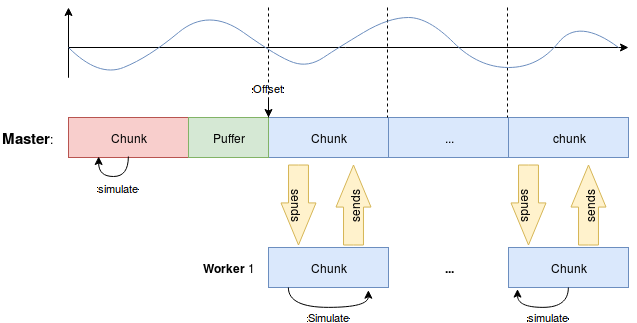
\includegraphics[width=1\textwidth]{pictures/Master_Slave_Dia2.png}
	\caption{Visualisierung der Master und Threadbeziehung}
	\label{fig:Visu_Master_Worker}
\end{figure}